\chapter{Documento de Arquitetura} \label{documento_arquitetura}

\begin{center}
 {\large Documento de Arquitetura}\\[0.2cm]
 {BEViM}\\
 \end{center}
 
 \section*{Histórico de Alterações}
\begin{table}[h]
\centering
\begin{tabular}{|c|c|p{6cm}|p{5cm}|}
\hline
Data & Versão & Descrição & Responsável\\
\hline                               
21/10/2016 & 1.0 & Criação do documento. & Emilie Morais.\\
\hline
\end{tabular}
\end{table}

\section*{Introdução}
	
    O objetivo deste documento é estabelecer uma visão da arquitetura da aplicação Web e do servidor REST de modo a estabelecer 
    um padrão de projeto e possibilitar uma melhor modularização e manutenabilidade de todo o sistema. 

\section*{Representação da Arquitetura}

Na Figura \ref{fig:representacao_arquitetura} está representada a arquitetura da aplicação Web (lado esquerdo) e do
servidor REST que é executado na Raspberry (lado direito). Ambas as aplicações estão estruturadas em camadas. 

\begin{figure}[!ht]
\centering
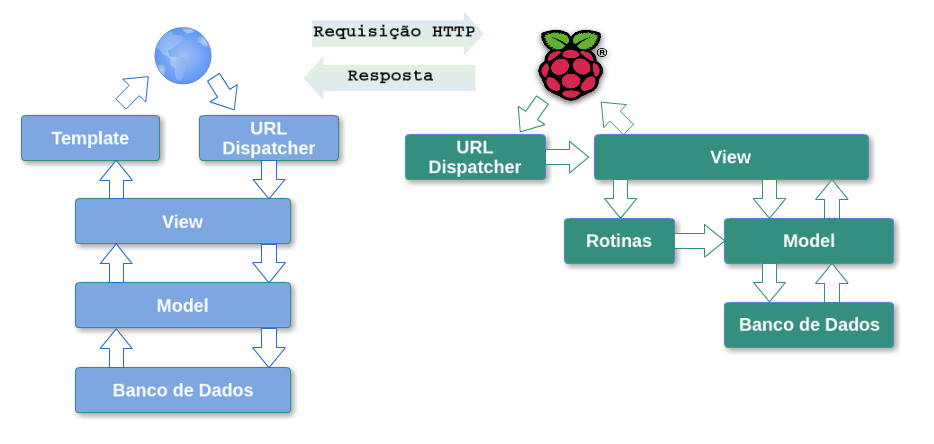
\includegraphics[keepaspectratio=true,scale=0.5]{figuras/representacao_arquitetura.png}
\caption{Representação da arquitetura}
\label{fig:representacao_arquitetura} 
\end{figure} 

A aplicação Web está estruturada em 3 principais camadas de acordo com a arquitetura do Django. As camadas são \textit{Template}, 
\textit{View} e \textit{Model}.
Nos \textit{Templates} são definidos como os elementos serão apresentados, na \textit{View} como os elementos serão processados e na
\textit{Model} são descritos os elementos e há a interação com o banco de dados (MySQL). Na \textit{View} há a interação com o 
\textit{URL Dispatcher}, ou seja, as requisições realizadas através de uma URL se comunicam com uma \textit{view} estabelecida.

No servidor da Raspberry a arquitetura é semelhante. A aplicação Web realiza as requisições através das URLs estabelecidas e dessa
forma há a comunicação com a \textit{View}, que possui a mesma responsabilidade que na aplicação Web. O processamento estabelecido
na \textit{View} pode comunicar-se com as rotinas ou com as \textit{models}. As \textit{models} definem os elementos representados no servidor,
as rotinas são responsáveis por realizar a comunicação com a porta serial, enviando e coletando dados. Além disso também realizam o
parser para armazenamento dos dados coletados, interagindo assim com as \textit{models}. 



\section*{Visão Lógica}
    A aplicação Web é a interface de todo o sistema da bancada com o usuário. A forma como este usuário 
    visualiza os elementos dispostos é responsabilidade dos \textit{templates}. Conforme o usuário interage com a
    aplicação são realizadas requisições HTTP através do \textit{browser} com o uso das URLs. As quais estão relacionadas com
    \textit{views}, dessa forma definindo como essas requisições são processadas. O processamento dessas requisições comunicam-se
    com as \textit{models} da aplicação que por sua vez comunicam-se com o banco de dados. Algumas requisições realizadas na aplicação
    estabelecem comunicação com o servidor que é executado na Raspberry.
    
    No lado do servidor as requisições provenientes são recebidas através das URLs definidas e relacionadas com as \textit{views}. Nas
    \textit{views} estas requisições são processadas contemplando a comunicação com as \textit{models} e em alguns casos com as rotinas. 
    As rotinas são executadas abrindo, escrevendo ou lendo e fechando a porta serial. Os dados lidos são armazenados através da comunicação
    com a \textit{model} que por sua vez se comunica com o banco de dados. Os dados inseridos no banco de dados são encaminhados para a
    aplicação através das respostas das \textit{views}. 
  
    
\section*{Visão de Dados}

Para o desenvolvimento das aplicações foi modelado um Diagrama Entidade-Relacionamento, que está representado na Figura \ref{fig:visao_de_dados}.
Este diagrama representa as tabelas da aplicação Web. No servidor REST as tabelas são apenas: \textit{Sensor, Data, Acceleration,
Speed, Amplitude} e \textit{Frequency}.

\begin{figure}[!ht]
\centering
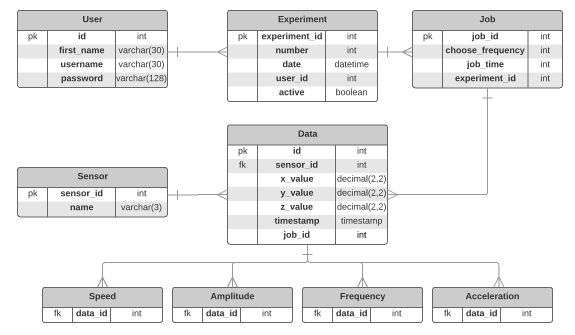
\includegraphics[keepaspectratio=true,scale=0.7]{figuras/visao_de_dados.png}
\caption{Visão de Dados}
\label{fig:visao_de_dados} 
\end{figure} 

    